% !Mode:: "TeX:UTF-8"
\section{课题主要研究内容及进度情况}

本课题将不确定性定义为“某个已经或即将发生的事件,它是的服务实际执行结果与预先达成的服务级别协议(Service Level Agreement, SLA) 之间产生了偏差”。服务执行中典型的不确定性包括:1) 某个服务环节未达到期望的质量(QoS) ;2) 某个服务环节执行失败;3) 客户需求发生变更或完全取消;4) 可用软件服务或服务资源的数量/价格发生波动;5) 外部商业环境或政策发生了变化,导致预设的服务流程失效;等等。从发生时间看,不确定性分为两种类型:已经发生并已造成影响的不确定性、明确知道将要发生但尚未发生的不确定性。

本课题将将站在中间人(broker)的角度,研究软件服务和业务服务的不确定性决策,首先建立服务不确定性决策模型,基于此模型采用软件服务实现不确定性决策,然后上升到业务服务的不确定性决策。

因此,将要研究的内容主要分为~4~个部分,它们之间的逻辑关系如图~\ref{main_content}~所示。

\begin{figure}[htbp]
    \centering
    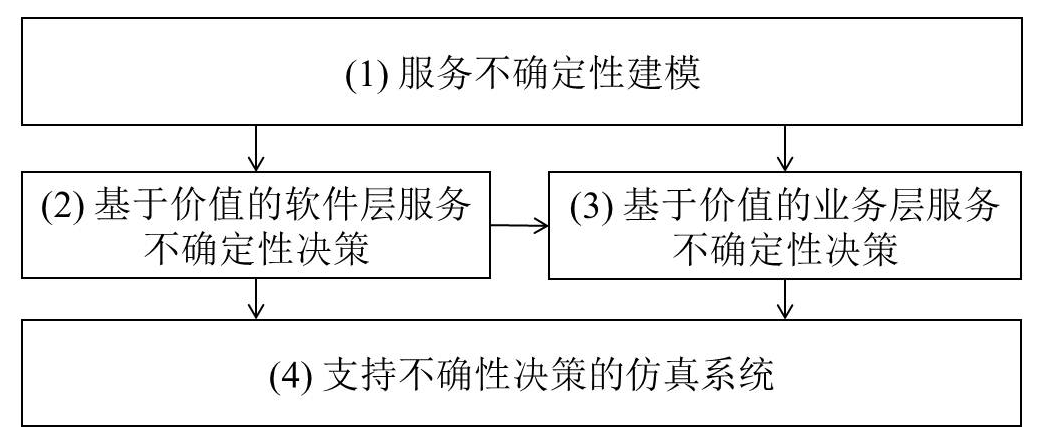
\includegraphics[width = 0.5\textwidth]{main_content}
    \caption{项目研究内容之间的逻辑关系}\label{main_content}
    \vspace{-1em}
\end{figure}

\setcounter{paragraph}{0}

(1) 服务不确定性建模。研究软件服务和业务服务的不确定性决策,建立服务不确定性决策模型。

(2) 基于价值的软件层服务不确定性决策。基于服务风险模型采用软件服务实现不确定性决策。

(3) 基于价值的业务层服务不确定性决策。将不确定性决策上升到业务服务层面,研究其决策方法。

(4) 支持不确定性决策的仿真系统。开发仿真系统对服务的不确定性进行仿真。

目前本课题已经完成不确定性建模,软件层面和业务层面的不确定性决策以及支持不确定性的仿真系统。工作量基本完成75\%,后续将对算法有效性和复杂性进行验证,最后进行论文的写作。


%\paragraph{服务不确定性建模}
%
%针对软件层服务,分别识别服务执行过程中可能面临的多种不确定性,对服务不确定性进行分类,并提出不确定性触发关系图~(Uncertainty Triggering Graph, UTG)~以描述多种不确定性事件之间可能存在的触发关系。同时,识别每种不确定性事件发生后可能的决策动作并将其分类,由于采用不同的动作其所获得的价值是同的,因此建立其收益/成本度量模型,来衡量不同决策动作之间的优劣,并研究决策出最优的动作。
%
%针对业务层服务,分别识别在用户需求和资源变化的不确定性进行分类,识别不同的不确定性,采取不同的决策方法,建立用户成本和服务提供者收益的价值度量模型,以衡量不同的决策之间的优劣,并研究作出收益最大化的决策动作。
%
%\paragraph{基于价值的软件层服务不确定性决策}
%
%根据服务执行中发生的具体不确定性,研究相应的不确定性触发关系图~(UTG)~的动态生成方法。提出基于动态~UTG~的不确定性影响范围及代价分析方法。识别优化目标(服务成功概率最大、时间延迟最小、成本最低),建立基于~Markov~决策过程~(MDP)~的不确定性优化决策模型并加以求解,生成对当前服务方案的最优改进策略。研究面向最小代价的运行时服务流程重组算法。
%
%\paragraph{基于价值的业务层服务不确定性决策}
%
%在业务层面,有比软件层面更灵活的需求和变化多端的外部环境。根据业务中用户需求和资源变化的不确定性,建立业务层面服务不确定性的决策模型并加以求解。研究用户成本最小化和服务提供者收益最大化的多目标优化决策方法。
%
%\paragraph{支持不确性决策的仿真系统}
%
%针对软件层和业务层的服务不确定性,开发一个服务不确定性决策仿真系统。此系统将软件层和业务层的服务不确定性事件,采用某种随机策略产生,使得服务执行至故障状态,并融入软件层和业务层的服务不确定性决策方法,采用不确定性决策算法对故障状态的服务流程进行最优动作的决策,使得服务方案得以继续执行。

%针对服务不确定性算法(基于~MDP~的服务自适应算法),采用传统的单步决策(贪心决策)与之进行对比,通过对比本课题的算法和传统算法的价值差(价值衡量),以及算法本身(时间复杂度和空间复杂度),从而证明本课题算法的有效性。

%\paragraph{不确性决策在海运物流中的应用验证}
%
%针对业务层面的服务,在以上两个软件层面的不确定性决策研究的基础之上,通过具体的海运业务示例,建立海运业务的不确定性的分类,研究针对其具体业务的决策方法,以及其不确定性事件之间可能存在的触发关系,建立其服务不确定性决策模型,并自动求解其针对当前业务执行状态的最优(成本最低/价值最高)策略。
%
%%对比其决策结果与传统人工决策结果,并对比其自动化决策效率和传统的人工决策效率之间的差值,将证明其决策效果的有效性和自动化决策的高效性。
%
%针对业务层面的不确定性,通过海运业务示例,分析归纳和对海运服务接口和产生海运不确定性事件进行分类。针对海运物流业务层面,开发一个具备海运物流不确定性事件自动化决策的应用系统。此系统将建立海运业务的具体业务执行流程,用~Web Service~提供海运业务的服务接口,从而使得海运业务IT化。系统将采用服务不确定性决策算法,针对业务层面进行服务不确定性决策,使之在人工决策上提供辅助功能。
